\section{Problem Statement}
\label{sec:problemStatement}

\begin{figure}[t]
\centering
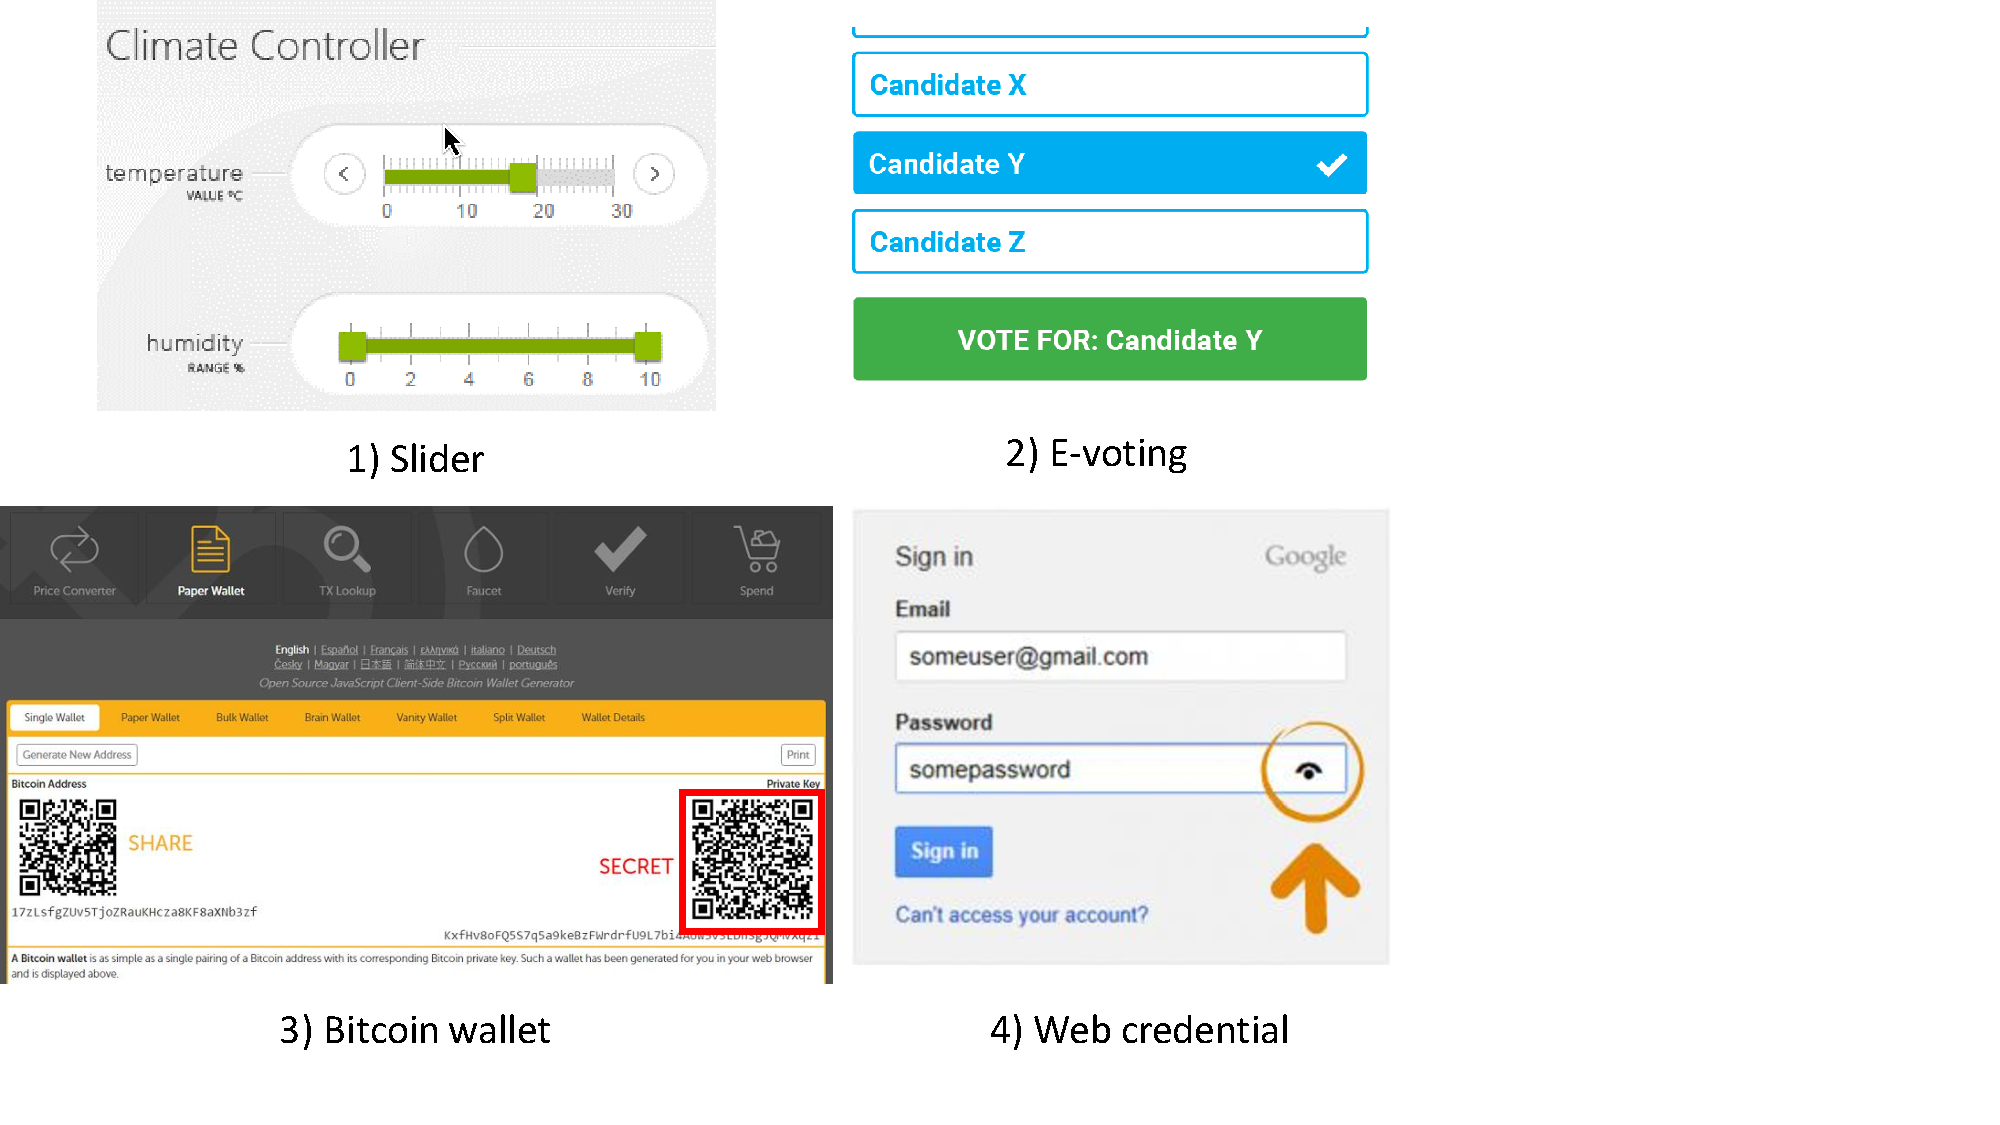
\includegraphics[trim={0 1cm 10cm 0}, clip, width=\linewidth]{motivation.pdf}
\caption{\textbf{\name motivating examples.} 1) Pointer based UI elements that sets parameters to remote safety-critical device, 2) E-voting where the voting privacy and integrity is critical, 3) Financial transactions such as bitcoin wallet that shows sensitive information such as the user's private key and 4) web appications that provide an option for the user to reveal credentials.}
\label{fig:motivation}
\centering
\end{figure}


\subsection{Motivation and Problem Statement}
Input integrity and privacy is a crucial problem when one assumes the attacker model where the attacker compromises host systems that include the hardware, the operating systems, and all the installed applications. Such an attacker model allows it not only to steal the sensitive information from the user but also alter them. Furthermore, the user is completely unprotected, she  cannot verify that her inputs are transfered to the server securely, or even have the guarantee that she is communicating with the legitimate server. The attacker can easily change system configurations (i.e.., install root certificates), alter user's transaction, or manipulate the user by showing false information on the screen. Figure~\ref{fig:motivation} provides four such cases where the secrecy and the integrity of the input and output data are crucial. Based on these examples we list 6 security properties that are provided by \name. We now discuss these security properties and corresponds them with the motivating example.

\begin{enumerate}
  \item \textbf{Input integrity.} In a case where the user provides input to a remote safety-critical system, input integrity is a crucial property that ensures that the command from the user reaches to the remote end-point without any modification by the malicious host system. Case 1 in Figure~\ref{fig:motivation} is a concrete example where input integrity is critical for the application to be work properly.
  \item \textbf{Input privacy.}  Input privacy is required if the malicious host wants to steal the sensitive information from the user. This involves the credentials for various web-service, financial information such as the credit card number, choice of the vote in the e-voting system. Cases 2,3,and 4 in Figure~\ref{fig:motivation} are the example where input privacy is needed.
  \item \textbf{Output integrity.} Output integrity is a critical component to ensure a secure display. This involves data coming from remote safety-critical devices, medical implants, financial data such as the bitcoin address, candidate list in the e-voting portal etc. Cases 1,2, and 3 in Figure~\ref{fig:motivation} are the potential scenarios where output integrity property is desirable.
  \item \textbf{Output privacy.} In many application scenarios, output privacy is required where the data sent from the remote end-point is privacy sensitive. Such includes the web credentials, candidate preference data in the e-voting, the private key of the bitcoin wallet etc. Example scenarios 2,3 and 4 in Figure~\ref{fig:motivation} require output privacy.
  \item \textbf{Activity privacy.} We define activity analogously to the user intention which is privacy sensitive in many application scenarios. One such concrete example is e-voting where voting privacy is of uttermost importance. Even if there is a system in place that provides input privacy, merely the fact that the user may hover her mouse over some candidates may reveal her candidate preference. Activity privacy is application specific and in most of the case, it dynamically preserves a part of the scene where the user activity is oblivious to the compromised host. 
\end{enumerate}


The problem that we try to solve is the following

\begin{enumerate}
  \item Integrity of the input device data (keyboard, mouse\ldots) and corresponds it to the frame data (of the display device) in the presence of an attacker-controlled host system.
  \item Installation of a single device, no change in any of the existing system/software or human interactions.
\end{enumerate}

\subsection{Attacker Model}

We assume the highly adversarial scenario where the attacker compromises the host system completely (OS, installed applications and hardware). The attacker also controlled the network. We only assume that it is a PPT-attacker, so he can not break crypto. Figure~\ref{fig:approachOverview} depicts the attacker model.

We only assume that the monitor, keyboard, mouse and the \device are trusted. Which is not unrealistic. The monitor, keyboard, and mouse have hardly any complex hardware. The TCB is very small.

\iffalse
\myparagraph{Advantages}

\begin{enumerate}
  \item The \device does not need to know the formatting/template of the page. As the \device only looks to the current mouse position, the structure of the page is somewhat irrelevant (?).
\end{enumerate}
\fi

\subsection{Limitations of the Known Solutions}

Previous research works such as IntegriKey~\cite{IntegriKey} uses a low-TCB embedded device to introduce a second factor for input integrity. Fidelius~\cite{Fidelius} uses raspberry pi's and Intel SGX to create a secure channel between the keyboard and the display device. By doing so Fidelius provides secure input and secure display for character-based input. We inspired from Fidelius to extend it even further to generic IO operations for a wider range of UI elements. Note that extending input devices, such as from a keyboard to a mouse is not a trivial task. Without proper analysis of each and every frame that the host system produces, it is not possible to track user intention. In our knowledge, \name is the first to provide such security properties including the activity privacy.
Moreover, \name achieves this in the absence of any TEE as the trust model of \name is significantly different. 


